\documentclass{article}

\usepackage[english]{babel}
\usepackage[letterpaper,top=2cm,bottom=2cm,left=3cm,right=3cm,marginparwidth=1.75cm]{geometry}
\setlength{\parindent}{0pt}

\usepackage{amsmath}
\usepackage{amsthm}
\usepackage{amssymb}
\usepackage{graphicx}
\usepackage{float}
\usepackage{listings}
\usepackage[colorlinks=true, allcolors=blue]{hyperref}
\usepackage{xcolor}

\lstset{
  basicstyle=\ttfamily\small,
  numbers=left,
  numberstyle=\tiny,
  stepnumber=1,
  numbersep=8pt,
  backgroundcolor=\color{gray!10},
  frame=single,
  rulecolor=\color{gray!60},
  tabsize=2,
  captionpos=b,
  breaklines=true,
  breakatwhitespace=true,
  showstringspaces=false,
  keywordstyle=\color{blue},
  commentstyle=\color{green!50!black},
  stringstyle=\color{orange},
}

\DeclareMathOperator{\VC}{VCdim}
\DeclareMathOperator{\supp}{supp}
\DeclareMathOperator{\sign}{sign}
\DeclareMathOperator{\Cov}{Cov}
\DeclareMathOperator*{\argmin}{arg\,min}

\newcommand{\EE}{\mathbb{E}}
\newcommand{\PP}{\mathbb{P}}
\newcommand{\cH}{\mathcal{H}}
\newcommand{\cD}{\mathcal{D}}
\newcommand{\cX}{\mathcal{X}}
\newcommand{\one}{\mathbf{1}}

\title{DSC 291: Learning Theory Assignment 5}
\author{Tongle Shen}

\begin{document}
\maketitle

\section{Part A: Sparse Halfspaces and Agnostic Hardness}

\subsection{Problem 1. Sample Complexity Versus Runtime}

Recall
$$
\cH_{d,k}
=
\left\{
x \mapsto \sign(\langle w,x\rangle)
:
w \in \mathbb{R}^d,\ \|w\|_0 \le k
\right\}.
$$
From Week 4 we already know
$$
\VC(\cH_{d,k})
=
O\!\left(
k\log\!\left(\frac{ed}{k}\right)
\right).
$$
Therefore, if an exact ERM oracle over $\cH_{d,k}$ were available, the Week 3 agnostic ERM theorem would give
$$
L_{\cD}(\widehat{h})
\le
\inf_{h\in \cH_{d,k}} L_{\cD}(h) + \varepsilon
$$
once
$$
n
=
O\!\left(
\frac{
\VC(\cH_{d,k})+\log(1/\delta)
}{
\varepsilon^2
}
\right)
=
O\!\left(
\frac{
k\log(ed/k)+\log(1/\delta)
}{
\varepsilon^2
}
\right).
$$
In particular, in the sparse regime this is polynomial in $k$, $\log d$, $1/\varepsilon$, and $\log(1/\delta)$.

The brute-force realizable algorithm from Week 4 is different. It enumerates all supports
$$
T\subseteq[d],
\qquad
|T|\le k,
$$
and for each support solves a halfspace feasibility problem in dimension $|T|$. Its runtime is
$$
\sum_{j=0}^k \binom{d}{j}\operatorname{poly}(n,j)
\le
\left(\frac{ed}{k}\right)^k \operatorname{poly}(n,k)
$$
up to constants.

\subsubsection{Why These Statements Are Fundamentally Different}

\textbf{Sample complexity} asks how many labeled examples are needed so that the ERM output generalizes once we can solve the optimization problem exactly.

\textbf{Runtime} asks how hard it is to implement that optimization problem.

So the VC bound is a statistical statement about estimation error, while the brute-force bound is a computational statement about support search. The Week 4 point was exactly that these two questions are logically separate: a class can have small agnostic sample complexity and still require an infeasible exact search procedure.

\subsection{Problem 2. NP-Hardness of Agreement}

I reduce from \textsc{Set Cover}.

\subsubsection{Set Cover Instance}

Start from a set-cover instance:
\begin{itemize}
\item universe $U=\{u_1,\dots,u_r\}$,
\item sets $A_1,\dots,A_q \subseteq U$,
\item budget $k$.
\end{itemize}
The question is whether there exists
$$
R\subseteq[q],
\qquad
|R|\le k,
$$
such that
$$
\bigcup_{j\in R} A_j = U.
$$

\subsubsection{Sparse-Halfspace Agreement Instance}

Set the ambient dimension to
$$
d=q,
$$
with one coordinate per set.

\textbf{Positive examples.}
For each set $A_j$, include the example
$$
p_j=e_j \in \mathbb{R}^q
$$
with label $+1$.

\textbf{Negative examples.}
For each universe element $u_i$, define
$$
a_i \in \{0,1\}^q,
\qquad
(a_i)_j = \one[u_i \in A_j].
$$
So $a_i$ records which sets cover $u_i$.

Choose
$$
M=q+1,
$$
and include $M$ copies of each negative example $(a_i,-1)$.

Finally set
$$
K := q-k+Mr.
$$

This construction is polynomial in the size of the set-cover instance.

\subsubsection{If the Set Cover Exists}

Assume there is a cover
$$
R\subseteq[q],
\qquad
|R|=s\le k,
$$
with
$$
\bigcup_{j\in R} A_j = U.
$$
Define
$$
w_j =
\begin{cases}
-1, & j\in R,\\
0, & j\notin R.
\end{cases}
$$
Then $\|w\|_0=s\le k$.

For each positive example $p_j=e_j$,
$$
\langle w,p_j\rangle = w_j.
$$
So $p_j$ is classified correctly iff $j\notin R$. Hence the number of correctly classified positive examples is
$$
q-s \ge q-k.
$$

Now fix a universe element $u_i$. Because $R$ covers $U$, some $j\in R$ satisfies $u_i\in A_j$, so
$$
\langle w,a_i\rangle
=
\sum_{j:u_i\in A_j} w_j
\le -1.
$$
Therefore every copy of $(a_i,-1)$ is classified correctly.

So the total agreement is at least
$$
(q-s)+Mr \ge q-k+Mr = K.
$$

\subsubsection{If Agreement at Least K Exists}

Conversely, suppose there exists a $k$-sparse vector $w$ whose classifier agrees with at least $K$ examples.

Let
$$
R := \{j : w_j < 0\}.
$$
Then
$$
|R| \le \|w\|_0 \le k.
$$

For the positive examples $p_j=e_j$, correctness requires
$$
\sign(w_j)=+1,
$$
which means $w_j\ge 0$. Hence every negative coordinate contributes one mistake on the positive side, so the total number of correctly classified positive examples is at most
$$
q-|R|.
$$

Now define the covered set
$$
\Cov(R) := \bigcup_{j\in R} A_j.
$$
If an element $u_i$ is not in $\Cov(R)$, then every set covering $u_i$ has nonnegative weight. Therefore
$$
\langle w,a_i\rangle
=
\sum_{j:u_i\in A_j} w_j
\ge 0,
$$
so every copy of $(a_i,-1)$ is misclassified. Thus only elements inside $\Cov(R)$ can contribute correctly classified negative examples. Hence the total agreement is at most
$$
q-|R| + M|\Cov(R)|.
$$

If $\Cov(R)\neq U$, then $|\Cov(R)|\le r-1$, so
$$
\text{agreement}
\le
q-|R|+M(r-1)
\le
q+M(r-1).
$$
Since $M=q+1>k$,
$$
q+M(r-1)
<
q-k+Mr
=
K.
$$
This contradicts the assumption that the agreement is at least $K$.

So necessarily
$$
\Cov(R)=U.
$$
Together with $|R|\le k$, this shows that $R$ is a set cover of size at most $k$.

\subsubsection{Conclusion of the Reduction}

I have shown:
\begin{itemize}
\item if the set-cover instance is a YES instance, then the constructed sparse-halfspace agreement instance has agreement at least $K$;
\item if the agreement instance has agreement at least $K$, then the original set-cover instance has a cover of size at most $k$.
\end{itemize}
Therefore deciding
$$
\mathrm{AGREEMENT}_{\cH_{d,k}}(S,K)
$$
is NP-hard when both $d$ and $k$ are part of the input.

\subsubsection{Implication for Agnostic Learning}

Week 5 proved the learner-to-agreement theorem: if a class family is efficiently properly agnostically PAC learnable, then its agreement problem lies in $\mathrm{RP}$.

Apply that theorem to the family
$$
\{\,\cH_{d,k} : d\ge 1,\ 1\le k\le d\,\}.
$$
If this family were efficiently properly agnostically PAC learnable with runtime polynomial in $d$, $k$, $1/\varepsilon$, and $\log(1/\delta)$, then
$$
\mathrm{AGREEMENT}_{\cH_{d,k}} \in \mathrm{RP}.
$$
But the reduction above shows that this agreement problem is NP-hard. Hence, assuming
$$
\mathrm{NP}\neq \mathrm{RP},
$$
the family $\cH_{d,k}$ is \emph{not} efficiently properly agnostically PAC learnable when $k$ is part of the input.

\subsection{Problem 3. Small Experiment}

\subsubsection{Artifacts}

The experiment code is in
$$
\texttt{hw5/code/sparse\_experiment.py},
$$
and the recorded numbers are in
$$
\texttt{hw5/code/experiment\_summary.json}.
$$
The plots are the PNG files under
$$
\texttt{hw5/figures/}.
$$

\subsubsection{Setup}

I compared two procedures.

\textbf{Exact sparse baseline.}
For very small samples, I used an exact proper search over $\cH_{d,k}$. The algorithm enumerates supports $T$ with $|T|\le k$, enumerates candidate subsets of examples that might be classified correctly, and checks each candidate by linear feasibility. So this baseline is exact, but only practical on tiny instances.

\textbf{Convex surrogate.}
I solved hinge-loss minimization with an $\ell_1$ radius constraint by linear programming. This is tractable and scales smoothly in these experiments, but it optimizes a surrogate over the larger $\ell_1$-bounded linear class rather than exact agreement over the $k$-sparse class.

\subsubsection{Runtime Scaling}

The first sweep fixed $k=2$ and $m=10$, and varied the ambient dimension $d$.
The median runtime of the exact sparse search increased from about
$$
0.442\text{ s at } d=4
$$
to about
$$
0.704\text{ s at } d=10\text{--}12,
$$
while the hinge LP stayed around
$$
0.0013\text{--}0.0018\text{ s}.
$$
The number of candidate supports in the exact search grew from
$$
\sum_{j=0}^2 \binom{4}{j}=11
\qquad\text{to}\qquad
\sum_{j=0}^2 \binom{12}{j}=79.
$$

\begin{figure}[H]
  \centering
  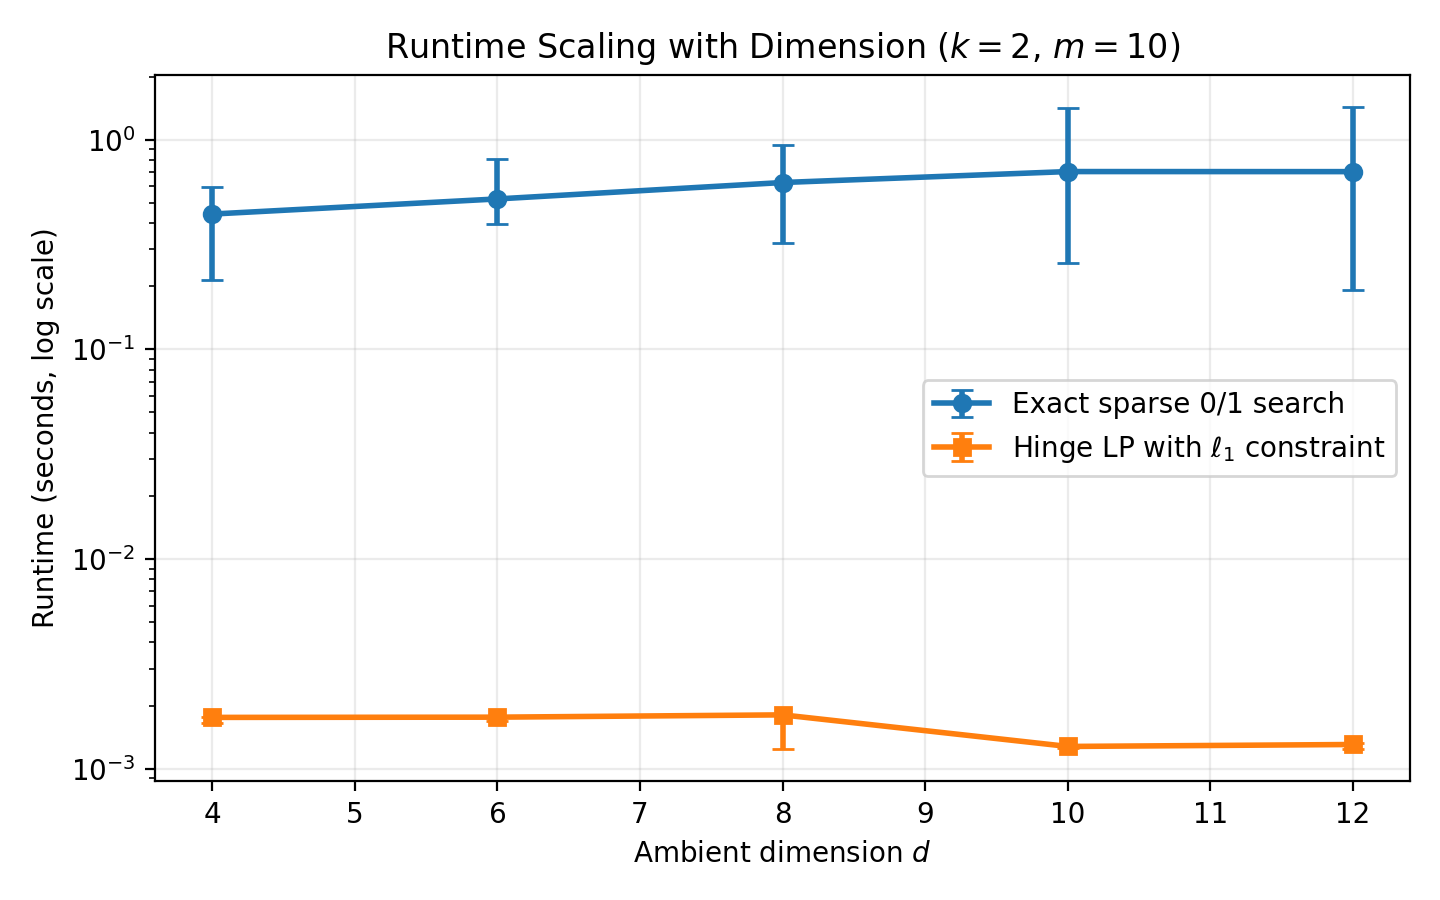
\includegraphics[width=1\linewidth]{figures/runtime_vs_dimension.png}
  \caption{Runtime comparison as the ambient dimension $d$ increases, with fixed sparsity budget $k=2$.}
  \label{fig:hw5_runtime_dimension}
\end{figure}

The second sweep fixed $d=12$ and $m=10$, and varied the sparsity budget. The exact sparse search rose from roughly
$$
0.279\text{ s at } k=1
$$
to roughly
$$
0.738\text{ s at } k=3,
$$
while the hinge LP again remained essentially flat near
$$
0.0013\text{ s}.
$$
This matches the support-count growth
$$
\sum_{j=0}^1 \binom{12}{j}=13,
\qquad
\sum_{j=0}^2 \binom{12}{j}=79,
\qquad
\sum_{j=0}^3 \binom{12}{j}=299.
$$

\begin{figure}[H]
  \centering
  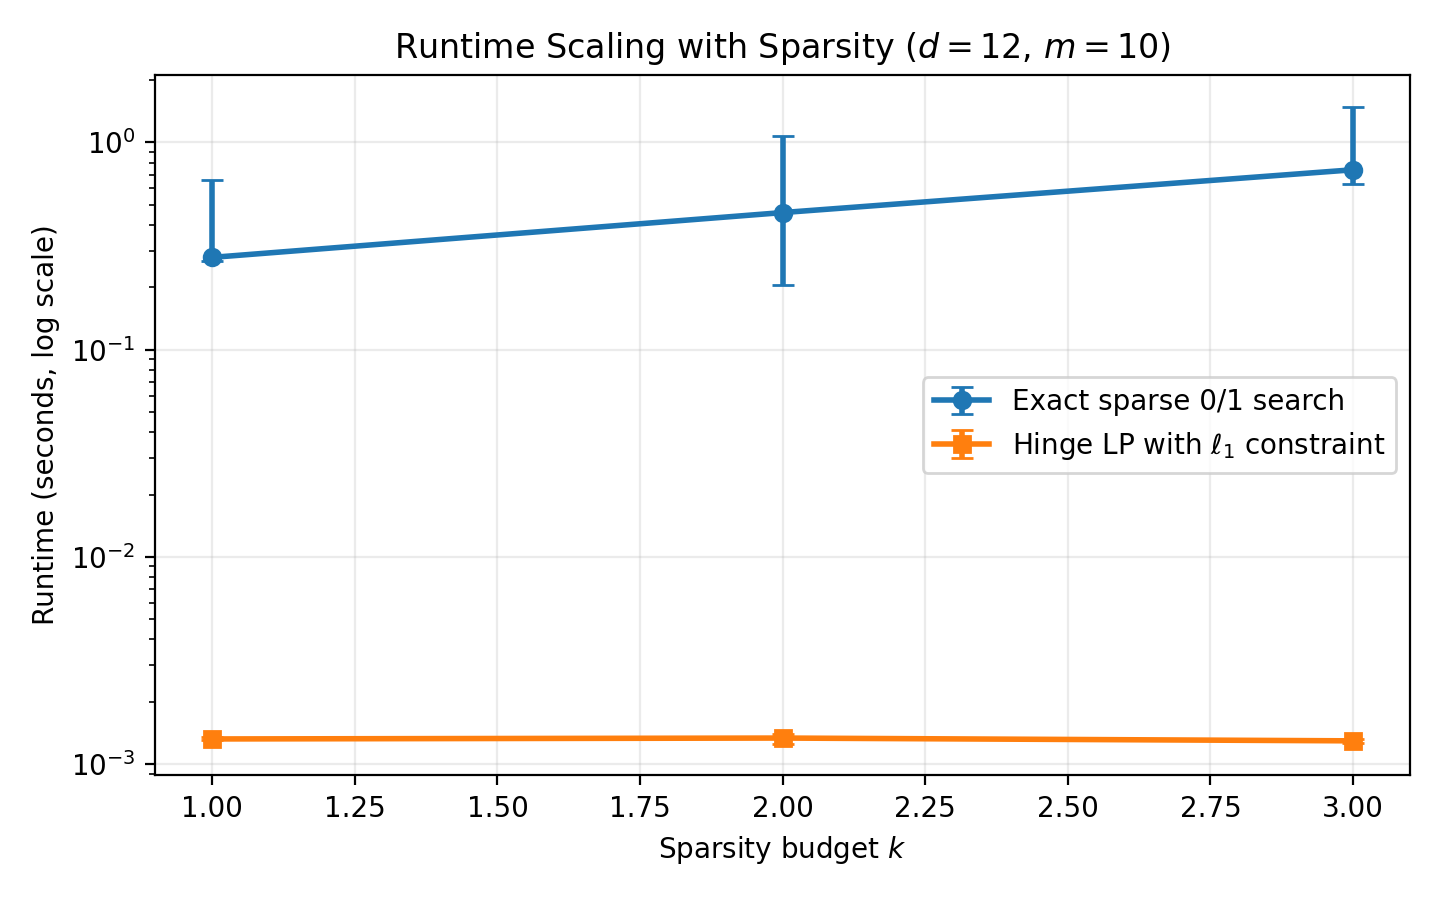
\includegraphics[width=1\linewidth]{figures/runtime_vs_sparsity.png}
  \caption{Runtime comparison as the sparsity budget $k$ increases, with fixed ambient dimension $d=12$.}
  \label{fig:hw5_runtime_sparsity}
\end{figure}

\subsubsection{Agreement Versus Surrogate Objective}

On a deliberately simple outlier dataset, the exact sparse baseline returned the zero vector and achieved training agreement
$$
1.000.
$$
The hinge LP instead chose
$$
w\approx -\frac{1}{12},
$$
which reduced the average hinge loss from
$$
1.000 \quad \text{to} \quad 0.774,
$$
but dropped the training agreement all the way to
$$
\frac{2}{7}\approx 0.286.
$$
So in this example the surrogate objective improves while the empirical $0/1$ objective becomes much worse.

\subsubsection{Does the Surrogate Return a Proper k-Sparse Classifier?}

In general, no. On a representative noisy dataset with target sparsity $k=2$, the exact sparse search returned a $2$-sparse classifier, while the hinge LP returned a vector with
$$
4
$$
nonzero coordinates. So the surrogate method was \emph{improper} relative to $\cH_{d,2}$.

On that same dataset, both methods had training agreement
$$
0.9,
$$
but the hinge LP obtained a lower hinge objective and a better validation agreement:
$$
0.660 \quad \text{versus} \quad 0.505.
$$
So the surrogate can trade exact sparsity for a larger linear class that may generalize better on some noisy instances.

\begin{figure}[H]
  \centering
  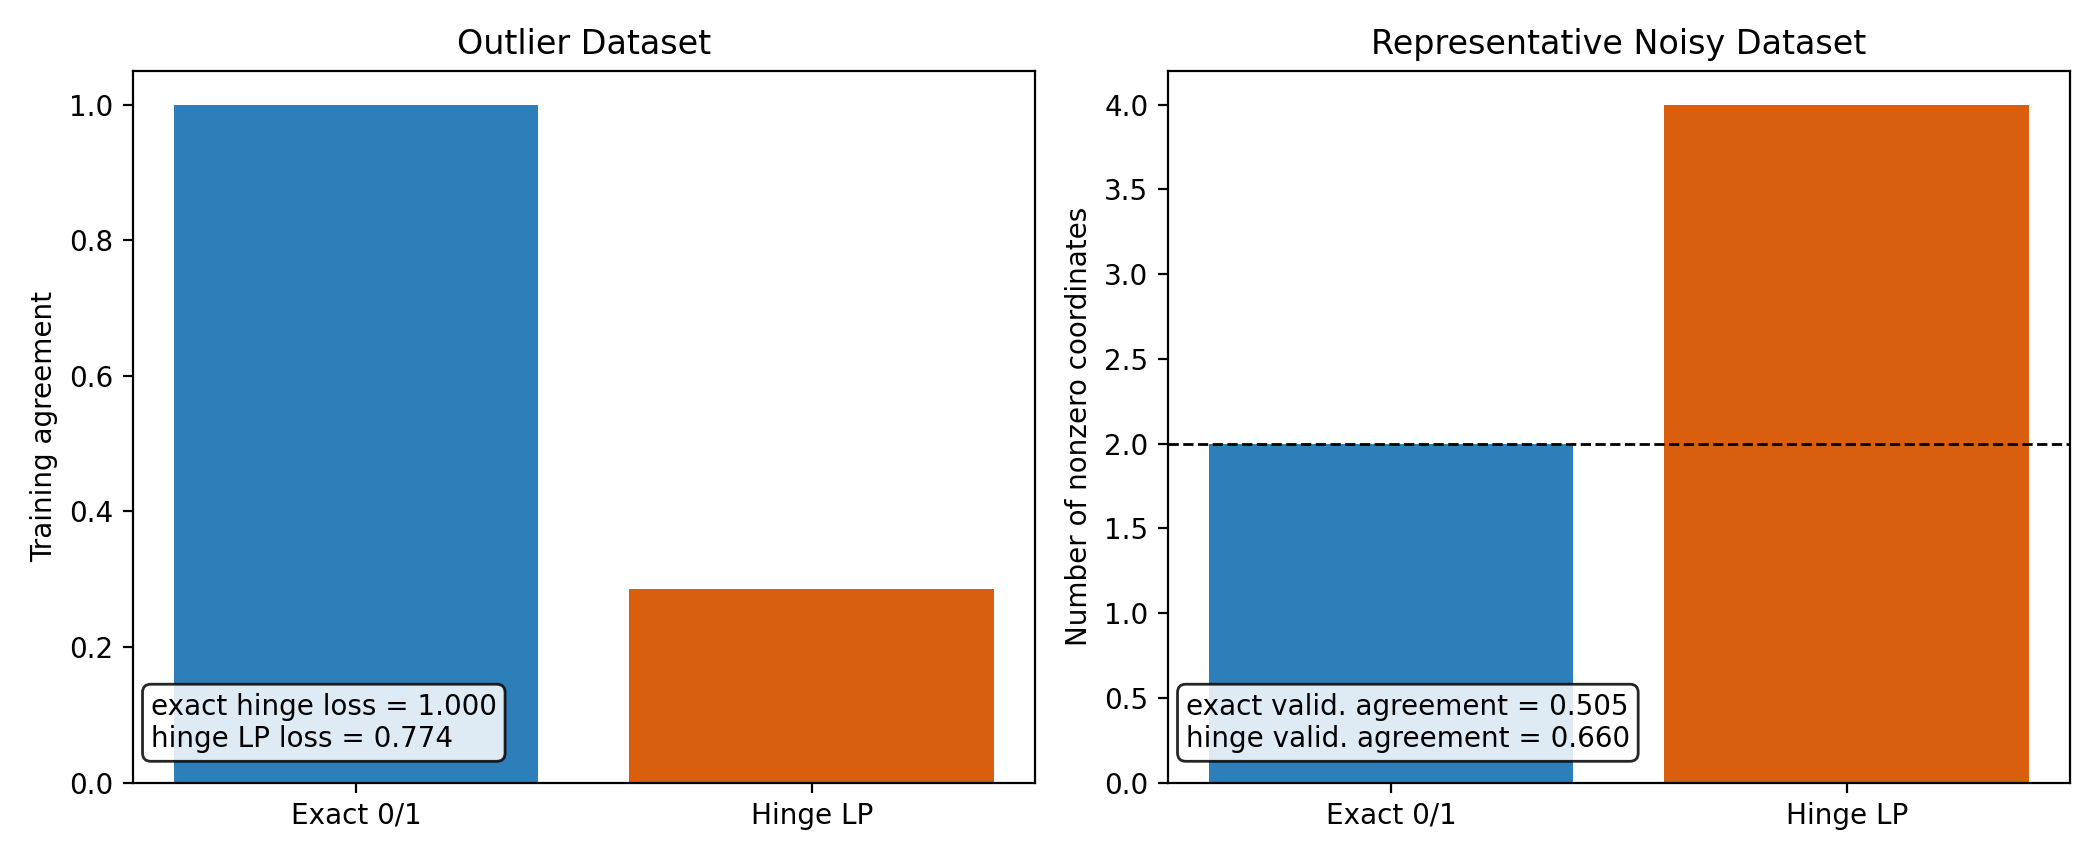
\includegraphics[width=1\linewidth]{figures/comparison_panels.png}
  \caption{Left: a surrogate-objective improvement can coexist with much worse empirical agreement. Right: the hinge LP can leave the proper $k$-sparse class by using more than $k$ nonzero coordinates.}
  \label{fig:hw5_comparison_panels}
\end{figure}

\subsubsection{Takeaway}

The experiment matches the Week 5 message. Exact agreement search over sparse halfspaces is a proper combinatorial optimization problem and becomes expensive quickly. Hinge-loss minimization is fast because it solves a convex relaxation over a larger class, but it optimizes the wrong objective for exact agreement and does not, in general, return a proper $k$-sparse classifier.

\newpage
\section{Part B: Surrogate Losses and the Fixed-Feature Barrier}

\subsection{Problem 1. Hinge ERM with an l1 Constraint}

The empirical hinge objective is
$$
\min_{\|w\|_1\le B}
\frac1m \sum_{i=1}^m (1-y_i\langle w,x_i\rangle)_+.
$$

\subsubsection{Linear-Program Formulation}

Write
$$
w_j = w_j^+ - w_j^-,
\qquad
w_j^+,w_j^- \ge 0,
$$
so
$$
\|w\|_1 = \sum_{j=1}^d (w_j^+ + w_j^-).
$$
Introduce slack variables
$$
\xi_i \ge 0
$$
for the hinge terms. Then the problem becomes
$$
\min_{w^+,w^-,\xi}
\frac1m \sum_{i=1}^m \xi_i
$$
subject to
$$
y_i\sum_{j=1}^d (w_j^+ - w_j^-)x_{ij} \ge 1-\xi_i
\qquad
\text{for } i=1,\dots,m,
$$
$$
\sum_{j=1}^d (w_j^+ + w_j^-)\le B,
$$
$$
w_j^+,w_j^- \ge 0,
\qquad
\xi_i \ge 0.
$$
This is a linear program.

\subsubsection{Why This LP Equals Hinge ERM}

Fix any $w$. The smallest feasible $\xi_i$ is exactly
$$
\xi_i = (1-y_i\langle w,x_i\rangle)_+.
$$
Therefore minimizing the LP objective is exactly the same as minimizing empirical hinge loss under the $\ell_1$ budget.

\subsubsection{Why This Is Not Empirical 0/1 Agreement over Sparse Halfspaces}

The tractable LP is \emph{not} the same problem as empirical agreement over sparse halfspaces for three reasons.

\textbf{Different objective.}
Agreement optimizes the number of correctly classified points. Hinge loss optimizes a convex upper bound that also penalizes low-margin correct predictions.

\textbf{Different feasible set.}
The LP uses
$$
\|w\|_1\le B,
$$
which does not enforce
$$
\|w\|_0\le k.
$$
So it searches a larger class.

\textbf{Improperness.}
Its output may be dense, hence it may lie outside $\cH_{d,k}$. This is exactly what happened in the experiment from Part A: the hinge LP used $4$ nonzero coordinates when $k=2$.

So hinge ERM is a computationally convenient surrogate problem, not the original agreement problem over $\cH_{d,k}$.

\subsection{Problem 2. A One-Dimensional Counterexample}

Let
$$
\PP[x=1]=1-p,
\qquad
\PP[x=-M]=p,
$$
with labels always $+1$, where
$$
0<p<\frac12,
\qquad
M>\frac{1-p}{p}.
$$
Consider predictors
$$
f_w(x)=wx.
$$

\subsubsection{Best 0/1 Error}

Because the label is always $+1$, the $0/1$ error is
$$
L_{\cD}^{0/1}(f_w)
=
(1-p)\one[w\le 0] + p\one[-Mw\le 0].
$$

If $w>0$, then
\begin{itemize}
\item $f_w(1)=w>0$, so $x=1$ is classified correctly,
\item $f_w(-M)=-Mw<0$, so $x=-M$ is misclassified.
\end{itemize}
Hence
$$
L_{\cD}^{0/1}(f_w)=p.
$$

If $w<0$, the roles reverse and
$$
L_{\cD}^{0/1}(f_w)=1-p.
$$

If $w=0$, then the margin is zero on both points, and with the assignment's convention for $0/1$ loss this counts as error on both, so
$$
L_{\cD}^{0/1}(f_0)=1.
$$

Therefore
$$
\inf_w L_{\cD}^{0/1}(f_w)=p,
$$
attained by every $w>0$.

\subsubsection{Population Hinge Risk}

The population hinge risk is
$$
L_{\cD}^{\mathrm{hinge}}(f_w)
=
(1-p)(1-w)_+ + p(1+Mw)_+.
$$
This is piecewise linear.

\textbf{Case 1: $w\le -1/M$.}
Then $(1+Mw)_+=0$, so
$$
L_{\cD}^{\mathrm{hinge}}(f_w)=(1-p)(1-w).
$$
This is decreasing in $w$ on this interval, so its minimum there is at
$$
w=-1/M.
$$

\textbf{Case 2: $-1/M\le w\le 1$.}
Both hinge terms are active, so
$$
L_{\cD}^{\mathrm{hinge}}(f_w)
=
(1-p)(1-w)+p(1+Mw)
=
1 + \bigl(pM-(1-p)\bigr)w.
$$
Because
$$
M>\frac{1-p}{p},
$$
we have
$$
pM-(1-p)>0,
$$
so this expression is increasing in $w$. Hence its minimum on this interval is also at
$$
w=-1/M.
$$

\textbf{Case 3: $w\ge 1$.}
Then $(1-w)_+=0$, so
$$
L_{\cD}^{\mathrm{hinge}}(f_w)=p(1+Mw),
$$
which is increasing in $w$.

Combining the three cases, every hinge-risk minimizer is
$$
w^*=-\frac{1}{M}.
$$

\subsubsection{Its 0/1 Error}

This minimizer is negative, so from the earlier case split,
$$
L_{\cD}^{0/1}(f_{w^*})=1-p.
$$
Thus every hinge-risk minimizer has $0/1$ error $1-p$.

\subsubsection{Conclusion}

Fix any $\varepsilon>0$ and any $\alpha<1$. Choose
$$
0<p<\min\{\varepsilon,1-\alpha\},
$$
and then choose
$$
M>\frac{1-p}{p}.
$$
Then
$$
\inf_w L_{\cD}^{0/1}(f_w)=p\le \varepsilon,
$$
but every hinge-risk minimizer satisfies
$$
L_{\cD}^{0/1}(f_w)=1-p>\alpha.
$$

So hinge minimization can be arbitrarily bad as a proxy for $0/1$ minimization.

\subsection{Problem 3. The Fixed-Feature Parity Barrier}

Let
$$
\chi_I(x)=\prod_{i\in I} x_i
\qquad
\text{for } I\subseteq[d],\ x\in\{-1,+1\}^d.
$$
Assume a fixed feature map
$$
\phi:\{-1,+1\}^d \to \mathbb{R}^D
$$
exactly realizes every parity:
$$
\chi_I(x)=\langle w_I,\phi(x)\rangle
\qquad
\text{for all } I\subseteq[d],\ x\in\{-1,+1\}^d.
$$

\subsubsection{Orthogonality of the Parity Matrix}

Define the matrix
$$
H\in \mathbb{R}^{2^d\times 2^d}
$$
whose rows are indexed by subsets $I\subseteq[d]$, whose columns are indexed by points $x\in\{-1,+1\}^d$, and whose entries are
$$
H_{I,x}=\chi_I(x).
$$

Take two subsets $I,J\subseteq[d]$. Then
$$
\chi_I(x)\chi_J(x)=\chi_{I\triangle J}(x),
$$
where $I\triangle J$ is the symmetric difference.

So the inner product of rows $I$ and $J$ is
$$
\sum_{x\in\{-1,+1\}^d} \chi_I(x)\chi_J(x)
=
\sum_{x\in\{-1,+1\}^d} \chi_{I\triangle J}(x).
$$
If $I=J$, then $I\triangle J=\varnothing$ and the sum equals
$$
2^d.
$$
If $I\neq J$, then $I\triangle J\neq\varnothing$. Pick some coordinate $t\in I\triangle J$. Pair each point $x$ with the point obtained by flipping only coordinate $t$. The parity $\chi_{I\triangle J}$ changes sign under this flip, so the terms cancel in pairs. Hence the sum is
$$
0.
$$

Therefore the rows of $H$ are pairwise orthogonal and nonzero, so
$$
\operatorname{rank}(H)=2^d.
$$

\subsubsection{Rank Factorization Bound}

Let
$$
W\in\mathbb{R}^{2^d\times D}
$$
have row $I$ equal to $w_I^\top$, and let
$$
\Phi\in\mathbb{R}^{D\times 2^d}
$$
have column $x$ equal to $\phi(x)$.

By the exact representation assumption,
$$
H=W\Phi.
$$
Hence
$$
\operatorname{rank}(H)
\le
\min\{\operatorname{rank}(W),\operatorname{rank}(\Phi)\}
\le D.
$$
Since $\operatorname{rank}(H)=2^d$, we obtain
$$
D\ge 2^d.
$$

\subsubsection{Matching Upper Bound}

Now define a feature map indexed by all subsets:
$$
\phi(x)
=
\bigl(\chi_J(x)\bigr)_{J\subseteq[d]}
\in \mathbb{R}^{2^d}.
$$
For a target parity $\chi_I$, choose
$$
w_I=e_I,
$$
the standard basis vector selecting coordinate $I$. Then
$$
\langle w_I,\phi(x)\rangle
=
\chi_I(x).
$$
So
$$
D=2^d
$$
is sufficient.

\subsubsection{Interpretation}

This proves the Week 5 fixed-feature barrier exactly. A fixed feature map can make the top-layer optimization convex, but if it must represent \emph{every} parity linearly, then its dimension must already be exponential. So the difficulty is not sample complexity or even the existence of linear predictors after lifting; it is that the lift itself must contain exponentially many interaction features.

\subsection{Problem 4. Same Predictors, Different Optimization Geometry}

Consider
$$
\mathcal{F}_{\mathrm{lin}}
=
\{x\mapsto \langle \beta,x\rangle : \beta\in\mathbb{R}^d\}
$$
and
$$
\mathcal{F}_{\mathrm{net}}
=
\{x\mapsto v\langle u,x\rangle : u\in\mathbb{R}^d,\ v\in\mathbb{R}\}.
$$

\subsubsection{Same Representable Functions}

Every function in $\mathcal{F}_{\mathrm{net}}$ is linear:
$$
v\langle u,x\rangle = \langle vu,x\rangle.
$$
So if we set
$$
\beta=vu,
$$
then
$$
x\mapsto v\langle u,x\rangle
=
x\mapsto \langle \beta,x\rangle.
$$

Conversely, every linear predictor in $\mathcal{F}_{\mathrm{lin}}$ belongs to $\mathcal{F}_{\mathrm{net}}$: given $\beta$, take
$$
u=\beta,
\qquad
v=1.
$$
Thus the two classes represent exactly the same set of predictors.

\subsubsection{Convexity of the Linear Parameterization}

For fixed data,
$$
L_{\mathrm{lin}}(\beta)
=
\frac1m \sum_{i=1}^m (\langle \beta,x_i\rangle-y_i)^2
$$
is a quadratic function of $\beta$ with Hessian
$$
\frac{2}{m}\sum_{i=1}^m x_i x_i^\top,
$$
which is positive semidefinite. Therefore $L_{\mathrm{lin}}$ is convex.

\subsubsection{Nonconvexity of the Factorized Parameterization}

By contrast,
$$
L_{\mathrm{net}}(u,v)
=
\frac1m \sum_{i=1}^m (v\langle u,x_i\rangle-y_i)^2
$$
is generally nonconvex in $(u,v)$ because of the bilinear product $vu$.

A concrete one-dimensional example already shows this. Take $d=1$, $m=1$, and the single sample
$$
(x_1,y_1)=(1,1).
$$
Then
$$
L_{\mathrm{net}}(u,v)=(uv-1)^2.
$$
Now compare
$$
(u_1,v_1)=(1,1),
\qquad
(u_2,v_2)=(-1,-1).
$$
Both satisfy
$$
L_{\mathrm{net}}(u_1,v_1)=L_{\mathrm{net}}(u_2,v_2)=0.
$$
But their midpoint is
$$
\left(\frac{u_1+u_2}{2},\frac{v_1+v_2}{2}\right)=(0,0),
$$
and
$$
L_{\mathrm{net}}(0,0)=1.
$$
So the midpoint has larger loss than the average endpoint loss:
$$
L_{\mathrm{net}}(0,0)
>
\frac12 L_{\mathrm{net}}(u_1,v_1)+\frac12 L_{\mathrm{net}}(u_2,v_2).
$$
Hence $L_{\mathrm{net}}$ is not convex.

\subsubsection{Global Minimizers Correspond}

Suppose $\beta^*$ minimizes $L_{\mathrm{lin}}$. Take any factorization
$$
\beta^*=vu.
$$
Then
$$
L_{\mathrm{net}}(u,v)
=
L_{\mathrm{lin}}(\beta^*),
$$
which is the minimum possible value. So every factorization of a globally optimal linear predictor is a global minimizer of the two-layer objective.

\subsubsection{Lesson}

Representational power and optimization geometry are different issues. The two parameterizations express exactly the same predictors, but the unfactorized linear parameterization gives a convex problem, while the factorized two-layer parameterization introduces symmetries and bilinear interactions that make optimization nonconvex. So changing the parameterization can make optimization much harder even when the hypothesis class itself does not change at all.

\newpage
\section{Part C: AI Usage Report}

I used AI for three parts of this assignment: structuring the sparse-halfspace hardness proof, checking the algebra in the one-dimensional hinge counterexample, and scaffolding the small experiment plus its LaTeX integration.

\textbf{Accepted suggestions.}
I accepted the suggestion to organize the \textsc{Set Cover} reduction into the two directions ``cover $\Rightarrow$ large agreement'' and ``large agreement $\Rightarrow$ cover,'' because that made the role of the repeated negative examples transparent. I also accepted the suggestion to prove the parity lower bound by a rank factorization
$$
H=W\Phi
$$
instead of by a longer linear-independence argument. For the experiment, I accepted the suggestion to compare an exact proper sparse baseline against an $\ell_1$-constrained hinge LP, because that matched the Week 5 contrast between proper combinatorial ERM and convex surrogate optimization.

\textbf{Rejected or modified suggestions.}
I rejected an early suggestion that hinge-loss minimization with an $\ell_1$ bound ``solves'' sparse ERM. That is false: the objective is different, and the output can be dense. I also modified an early runtime experiment because it depended too much on lucky early stopping in the exact search; I replaced it with a more stable exact-search comparison and reported medians from repeated runs.

\textbf{Verification.}
I checked the proofs against the Week 5 handout and re-derived the key inequalities by hand, especially the condition
$$
M>\frac{1-p}{p}
$$
in the hinge counterexample and the threshold
$$
K=q-k+Mr
$$
in the reduction. For the experiment, I ran
$$
\texttt{python hw5/code/sparse\_experiment.py}
$$
inside the active \texttt{ai4lt} environment, inspected the generated JSON summary and PNG figures, and then rebuilt the PDF with \texttt{pdflatex}.

\textbf{Five recent workflow updates.}
\begin{enumerate}
\item I added \texttt{scipy} to \texttt{environment.yml} so LP-based experiments can be reproduced in the tracked Conda environment.
\item I kept all experiment code under \texttt{hw5/code/} and all plots under \texttt{hw5/figures/} to match the repo convention.
\item I recorded experiment outputs in a JSON file before quoting any numbers in LaTeX, so the writeup stays tied to reproducible artifacts.
\item I used a compile pass after the main draft and again after cleanup edits, which caught the usual PDF-bookmark issues early.
\item I now explicitly separate comparator, feasible set, and proper-versus-improper status whenever a surrogate method appears, because that was the main conceptual source of confusion in this assignment.
\end{enumerate}

\end{document}
